\begin{savequote}[75mm] 
All our history hidden, ain't no liberty given\\
We all fit the description of what the documents written
\qauthor{``Land of the Free''- Joey Bada\$\$} 
\end{savequote}

\chapter{Inferring Artist Influence with the Document Influence Model}
As a first content-based approach to inferring artist influence based on audio samples, we used the Document Influence Model (DIM) \cite{gerrish2010language} developed by Gerrish and Blei.

The Document Influence Model is an extension to traditional topic modeling which allows for the evolution of topics over time. Though originally developed for text documents, the DIM also makes sense in the context of music since music consists of multiple genres and subgenres which also mix and evolve over time. Furthermore, since this model has previously been applied in a similar way by Shalit et al. \cite{shalit2013modeling} we used it as a baseline check for our data pipeline.

\section{Model}
The DIM is a probabilistic time series model with the following three components:
\begin{enumerate}
    \item Latent Dirichlet Allocation (LDA) \cite{blei2003latent} fit separately on each time epoch, with each epoch corresponding to a year of song release in this case.
    \item Time evolution: Each topic evolves with time, linking the different epochs.
    \item Song-topic influence factor: Each song has a hidden associated influence factor for each topic whose value is revealed via posterior influence. Therefore, in this model influential songs are defined as songs that ``pull'' the language of later songs in their topic in their direction.
\end{enumerate}

Formally, we have a corpus of $D$ songs (documents) where each song $d \in \{1...D\}$ consists of a set of $N_d$ musical words $w_1^d,...,w_{N_d}^d$ drawn from a vocabulary of total size $W$. Each song belongs to one of $T$ time epochs (song release year, though we also experimented with using the start year of the artist's career), and we assume $K$ total topics.

Each word $w_n^d$ is generated from one topic $k \in \{1...K\}$, with topic assignment indicated by the variable $z_{n,k}^d$. Since each song is a bag-of-words representation over the topics, then therefore $\frac{1}{N_d} \sum_{n=1}^{N_d} z_{n,k}^d$ represents the proportion of each topic $k$ in song $d$.

The probabilistic model used is defined as follows:
The word distribution at time $t$ for topic $k$ is given by a $W$-dimensional natural parameter vector $\beta_{k, t}$, with the probability of a word $w$ given by the softmax transformation:

$$p(w|\beta_{k, t}(w)) \propto exp(\beta_{k, t}(w))$$

The topic-term distribution drifts over time via the stationary autoregressive process
$$\beta_{k, t+1}|\beta_{k, t} \sim \mathcal{N}(\mu_{k,t}, \sigma^2I)$$
where $\sigma^2$ is the transition variance and
\begin{align*}
    \mu_{k,t} &= \beta_{k,t} + exp(-\beta_{k,t})\sum_{d} \ell_k^d \cdot \kappa(t, \tau(d))\sum_n w_n^d z_{n,k}^d
\end{align*}
where the first component of the sum is the topic-term distribution in the previous time-epoch and the second component of the sum is the sum of the songs in the previous epochs, scaled by their influence score and a time-delay kernel (in this case, a log-normal kernel was used), denoted by $\kappa(t, \tau(d))$ with $\tau(d)$ representing the release year of the song. $w_n^d$ is an indicator defined to be $1$ if the $n$th word $w_n$ appears in document $d$ and $0$ otherwise. Each song is given a normally distributed topic-influence score $\ell_k^d$ which denotes how much the language of topic $k$ drifts in the direction of the language of song $d$.

\begin{figure}[H]
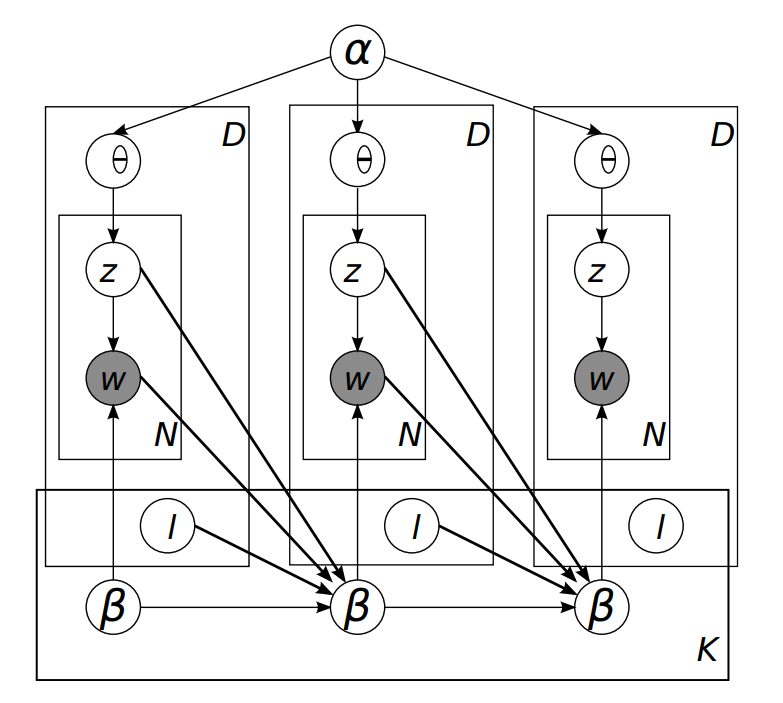
\includegraphics[width=\textwidth]{figures/dim_plate.png}
\caption{Plate diagram of the Document Influence Model}
\end{figure}

As the exact posterior distribution is intractable, Gerrish \& Blei derived a variational approximation using Kalman filters \cite{gerrish2010language}, the details of which are omitted here. 

Posterior inference enables us to estimate the topic-influence scores $\ell_k^d$ (Note: $\ell$ is written as $l$ in the plate diagram in figure 4.1.1), which is the key variable of interest. We defined the influence of each song as $\ell^d = \max_{\substack{k}} \ell_k^d$, and for each artist $a \in \{1...A\}$, we set the influence for the artist $\ell^a$ as the average over all $\ell^d$ corresponding to songs by that artist. 

\section{Experimental Setup}
\subsection{Feature Representation}
As is generally the case with topic modeling, the DIM also requires that each song (document) be represented as a bag-of-words (BOW). Previously, Shalit et al. \cite{shalit2013modeling} used features from the publicly available Million Songs Dataset, and also engineered music domain specific features such as max. loudness, chroma and timbre. 

Since we did not use the Million Songs Dataset, instead relying upon raw audio scraped directly from AllMusic to maximize overlap with the ground truth influence graph, we had to generate audio features ourselves. To this end, we used a common procedure \cite{mcfee2012learning} for generating a bag-of-words representation for the MFCC representation of each audio track. For reference, the MFCC representation for each audio file was a (number\_of\_features, number\_of\_frames) array of floats with each frame corresponding essentially to a timestep. In our case, we had a $(13, 1298)$ array for each MFCC representation, corresponding to the first 13 MFCC coefficients over 1298 frames (approximately 30 seconds). The bag-of-words generation procedure used is as follows:

\begin{enumerate}
    \item Normalize each MFCC coefficient by subtracting the mean and dividing by the standard deviation across the entire audio dataset for that coefficient.
    \item Cluster all normalized 13-dimensional frames across the entire audio dataset using minibatch $k$-means \cite{sculley2010web}. $k$ corresponds to the desired dimensionality (vocabulary size) of the end bag-of-words representation.
    \item For each normalized MFCC representation, quantize each frame by assigning the frame to the nearest cluster center, tallying the counts of assignments for each cluster over all frames to obtain a bag-of-words.
\end{enumerate}

\subsection{Model Fitting}
Since inference for the Document Influence Model with the scale of data that we used was too RAM-intensive, we performed model fitting on Harvard's Odyssey cluster. Specifically, we fit the DIM on 125,965 total songs compared to the 24,941 songs used by Shalit et al. The breakdown of number of songs for each epoch (year of release) can be seen in the figure below. 

\begin{figure}[H]
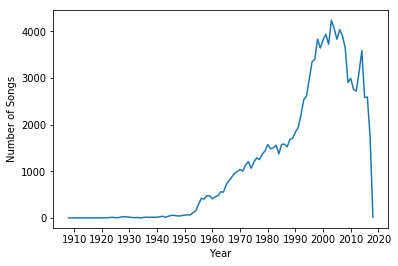
\includegraphics[width=\textwidth]{figures/dim_songs_epoch.png}
\caption{Number of songs per year used to fit DIM}
\end{figure}

In our experiments, we tried out bag-of-words sizes of 500 and 1000 and number of topic settings 1, 5 and 10. Due to the amount of time it took to generate features according to the procedure described in 4.2.1, we did not optimize for the selection of $k$ in $k$-means for our bag-of-words size, though strategies such as the elbow method or the gap statistic \cite{tibshirani2001estimating} certainly could have been used.

\section{Results}
\subsection{Correlation with AllMusic Influence Graph}
To evaluate the model, we calculated the Spearman correlation coefficient between artist influence score according to the unsupervised model and artist out-degree from the ground-truth influence graph that we scraped. The results for several configurations are summarized in the table below (all statistically significant with $p < 0.05$):

\begin{table}[H]
\centering
\caption{Correlation of DIM Influence with AllMusic Outdegree}
\label{my-label}
\begin{tabular}{|l|l|l|}
\hline
BOW Size & Number of Topics & Correlation \\ \hline
500      & 1                & 0.1303        \\ \hline
500      & 5                & 0.1687      \\ \hline
500      & 10               & 0.1733    \\ \hline
1000     & 1                & 0.1052      \\ \hline
1000     & 5                & 0.1819      \\ \hline
1000     & 10               & 0.1691      \\ \hline
\end{tabular}
\end{table}

\subsection{Most Influential Artists from Best DIM Model}
We computed the top 25 most influential artists according to the highest-correlated model (BOW Size 1000, 5 topics) in terms of $\ell^a$ (as defined in section 4.1), filtering for artists with out-degree greater than 100 in the ground truth graph. We applied this filtering in order to counteract noise in the model fitting process from some time epochs having very few total songs, which led to some artists with very low out-degree having an inflated value of $\ell^a$. To reemphasize however, the DIM is an unsupervised model with no out-degree information or other metadata used during the fitting process, just the BOW feature representations of song audio.

\begin{table}[H]
\centering
\caption{Most influential artists according to best DIM Model}
\label{my-label}
\begin{tabular}{rl}
\hline
   Rank & Artist          \\
\hline
      1 & Bob Marley      \\
      2 & Parliament      \\
      3 & Stevie Wonder   \\
      4 & Frank Zappa     \\
      5 & Prince          \\
      6 & Louis Armstrong \\
      7 & The Band        \\
      8 & Curtis Mayfield \\
      9 & The Clash       \\
     10 & Ray Charles     \\
     11 & Kiss            \\
     12 & Funkadelic      \\
     13 & The Yardbirds   \\
     14 & Tom Waits       \\
     15 & The Who         \\
     16 & Otis Redding    \\
     17 & Elvis Costello  \\
     18 & MC5             \\
     19 & T. Rex          \\
     20 & Kraftwerk       \\
     21 & New Order       \\
     22 & James Brown     \\
     23 & Alice Cooper    \\
     24 & Buddy Holly     \\
     25 & Ella Fitzgerald \\
\hline
\end{tabular}
\end{table}

The artists in the table above do not necessarily have the highest out-degrees (compare with table 3.1.1). We see that like PageRank (table 3.1.2), the DIM identifies Louis Armstrong as a highly influential artist despite his out-degree not being in the top 25. Overall, qualitatively this list looks reasonable: it includes pioneers of jazz (Louis Armstrong, Ella Fitzgerald), rock (Buddy Holly, The Yardbirds), electronic (Kraftwerk), funk (Parliament and its sister act Funkadelic), soul (Otis Redding, Curtis Mayfield, James Brown, Ray Charles) and punk (MC5). Obviously, these results are not without caveats: the filtering by out-degree step above does introduce bias and the relative rankings of artists is by no means definitive (Is Bob Marley \textit{really} the most influential artist of all time, across all genres?).

% TODO: Add Baseline
% TODO: Topic breakdown by genre/style
% TODO: Add some examples of influential songs (denoised)?

\section{Discussion}
\subsection{Comparison to Shalit et al.}
Fitting the Document Influence Model on the audio dataset we gathered and through the bag of words feature extraction procedure described above, we achieve comparable results to what Shalit et al. obtained. For reference, Shalit et al. used audio features from the Million Songs Dataset in addition to additional engineered features to yield a larger bag-of-words vocabulary size of 5033, a smaller audio dataset of around 25k songs, and 12 total time epochs, achieving a top Spearman rank correlation of 0.15 using a 10 topic model.

In contrast, our best correlation was achieved with a 5 topic model with a bag of words size of 1000 and features generated by ourselves using the procedure described in section 4.2.1, with the slight boost in correlation probably attributable to the increase in amount of data.

\subsection{Limitations}
Though it yielded respectable results, a key limitation of the bag-of-words feature extraction we used is that much information is lost in the various stages of the feature extraction pipeline. First, in order to make clustering computationally tractable, we employ a MFCC feature representation, which is lossier than a mel-spectrogram representation. Next, we apply minibatch $k$-means, which produces lower-quality clusterings than standard $k$-means, which itself is a heuristic that is not guaranteed to find a globally optimal clustering in terms of minimizing loss (in fact, the $k$-means clustering problem in general is NP-hard). Finally, our resulting bag-of-words representation does not capture the rich temporal structure and substructure of music since it is merely a count summary that does not take order into account. Another limitation is that the DIM yields an influence score for each document on a per-topic basis, as opposed to the artist-to-artist level. With these issues of (1) a need for richer feature representations and (2) artist-to-artist influence modeling capacity in mind, we turn to exploring a deep learning approach to modeling artist-to-artist influence in the next chapter.